\documentclass[a4paper]{article}

% Language and font encodings
\usepackage[english]{babel}
\usepackage[a4paper,top=3cm,bottom=2cm,left=3cm,right=3cm,marginparwidth=1.75cm]{geometry}
\usepackage{amsmath}
\usepackage{graphicx}
\usepackage{tabularx}
\usepackage{natbib}
\usepackage{subcaption}
\usepackage[colorinlistoftodos]{todonotes}
\usepackage[colorlinks=true, allcolors=blue]{hyperref}
\usepackage{wrapfig}
\DeclareMathAlphabet{\pazocal}{OMS}{zplm}{m}{n}
\usepackage{setspace}
\usepackage{hyperref}
\hypersetup{
    colorlinks=true,
    linkcolor=blue,
    filecolor=magenta,      
    urlcolor=cyan,
}
\urlstyle{same}

%%%%%%%%%%%%%%%%%%%%%%%%%%%%%%%%%%%%%%%%%%%%%%%%%%%%%%%%%%%%%%%%%%%%%%%%%%%%%%%%

\begin{document}

\begin{center}
  {\Large \bf Milestone 4: Computing the CMB Power Spectrum. }\\[4ex]
  {\large Daniel Herman}\\[4ex]
  \normalsize
  \today
  \vspace*{8ex}
      
  \begin{minipage}[t]{12cm}
      
  {\bf Abstract.} Using the results from the previous milestones, we compute the angular CMB power spectrum using line-of-sight integration techniques. We use the values computed in Milestone 3 to calculate the source function of the power spectrum.
  
  \vspace*{8ex}
  \end{minipage}

\end{center}

\section{Introduction}\label{sec:intro}

In this milestone we utilize the physical quantities computed in the previous milestones to compute the CMB power spectrum. Using line-of-sight integration techniques as described in (SOURCE), we can represent the size of perturbation growths in a simple plot with only one dependent variable. This variable, $l$, represents the angular scale size of the perturbation in question, similar to the Fourier space variable $k$ used in Milestone 3.\\

We compare the results of our computation to that of the latest PLANCK 2015 data release power spectrum, and adjust cosmological parameters to attempt to get the best fit. Altering these variables will help us get an intuition into the effects of these different parameters on the structure growth of the universe.

\section{Methods}\label{sec:meth}

In the same way as the previous 

As was mentioned above, we utilize the line-of-sight integration techniques described in (SOURCE). This method cuts down significantly on computation time because instead of evaluating the full temperature field in the multipoles computed in Milestone 3, we can instead evaluate the integral of the original equation for $\dot{\Theta}$. We will gloss over the exact details of determining this integral, but the expression for the transfer function $\Theta_l$ becomes

\begin{equation}\label{eq:transf}
\Theta_l(k,x=0) = \int_{-\infty}^0 \tilde{S}(k,x)j_l[k(\eta_0 - \eta)]dx
\end{equation}

where $\tilde{S}(k,x)$ is the source function, and $j_l$ is the spherical Bessel function which weights the integral for each $k$. The source function takes the form

\begin{equation}\label{eq:source}
\tilde{S}(k,x) = \tilde{g} \big[\Theta_0 + \Psi + \dfrac{1}{4}\Pi \big] + e^{-\tau}[\Psi' - \Phi'] - \dfrac{1}{k}\dfrac{d}{dx}(\pazocal{H}\tilde{g}v_b) + \dfrac{3}{4k^2}\dfrac{d}{dx} \big[\pazocal{H}\dfrac{d}{dx}(\pazocal{H}\tilde{g}\Pi) \big].
\end{equation}

where $\Pi = \Theta_2 + \Theta_2^P + \Theta_0^P$. Since we are doing a calculation neglecting the polarization, we can drop the second two terms.\\

We see that all of the terms present in the source function above have already been computed in previous milestones. Using the $k$ and $x$ values from evolution mod, we create a two-dimensional array of the source function. Before we begin our integration to solve for $\Theta_l$, we create a high-resolution two-dimensional grid of our source function utilizing two-dimensional splining techniques, with 5000 points for the $x$-grid and 5000 points for the $k$-grid.\\

\clearpage

Before we can integrate our source function, we calculate splined values for the spherical bessel function for the $l$ values we are interested in. Once this has been done, we begin integrating using a basic Riemann sum integral approach where we sum over $x$. The result, $\Theta_l(k)$, which we call the transfer function is necessary for our next calculation. In order to save a lot of time on repeating calculations, we save the calculated Milestone 3 variables and the splined spherical bessel function values to unformatted files which the program reads.\\

We now want to actually calculate the coefficients for the power spectrum itself. The expression for the angular power spectrum $C_l$ is as follows

\begin{equation}\label{eq:power}
C_l = \int_0^{\infty} \Big(\dfrac{ck}{H_0}\Big)^{n-1} \Theta_l^2(k) \dfrac{dk}{k}.
\end{equation} 

As done above concerning equation \ref{eq:transf}, we skip over the details of the derivation of this integral. For both equation \ref{eq:transf} and equation \ref{eq:power} we calculate the integrals using a simple Riemann sum technique where for the transfer function we sum over all $x$-values and for $C_l$ we sum over all $k$-values.

\section{Results}

In this section we look at the results for the transfer function $\Theta_l(k)$ and the integrand of the power spectrum for comparison to the plots in Callin. We also look at the regular angular power spectrum. At the end of this section, we vary differing parameters to compare with the most recent Planck power spectrum data and investigate how the different parameters affect the shape and behavior of the computed $C_l$.

\subsection{Transfer function}

In the figure below we have the transfer function for six different $l$ values.

\begin{figure}[ht]\label{fig:trans}
\centering
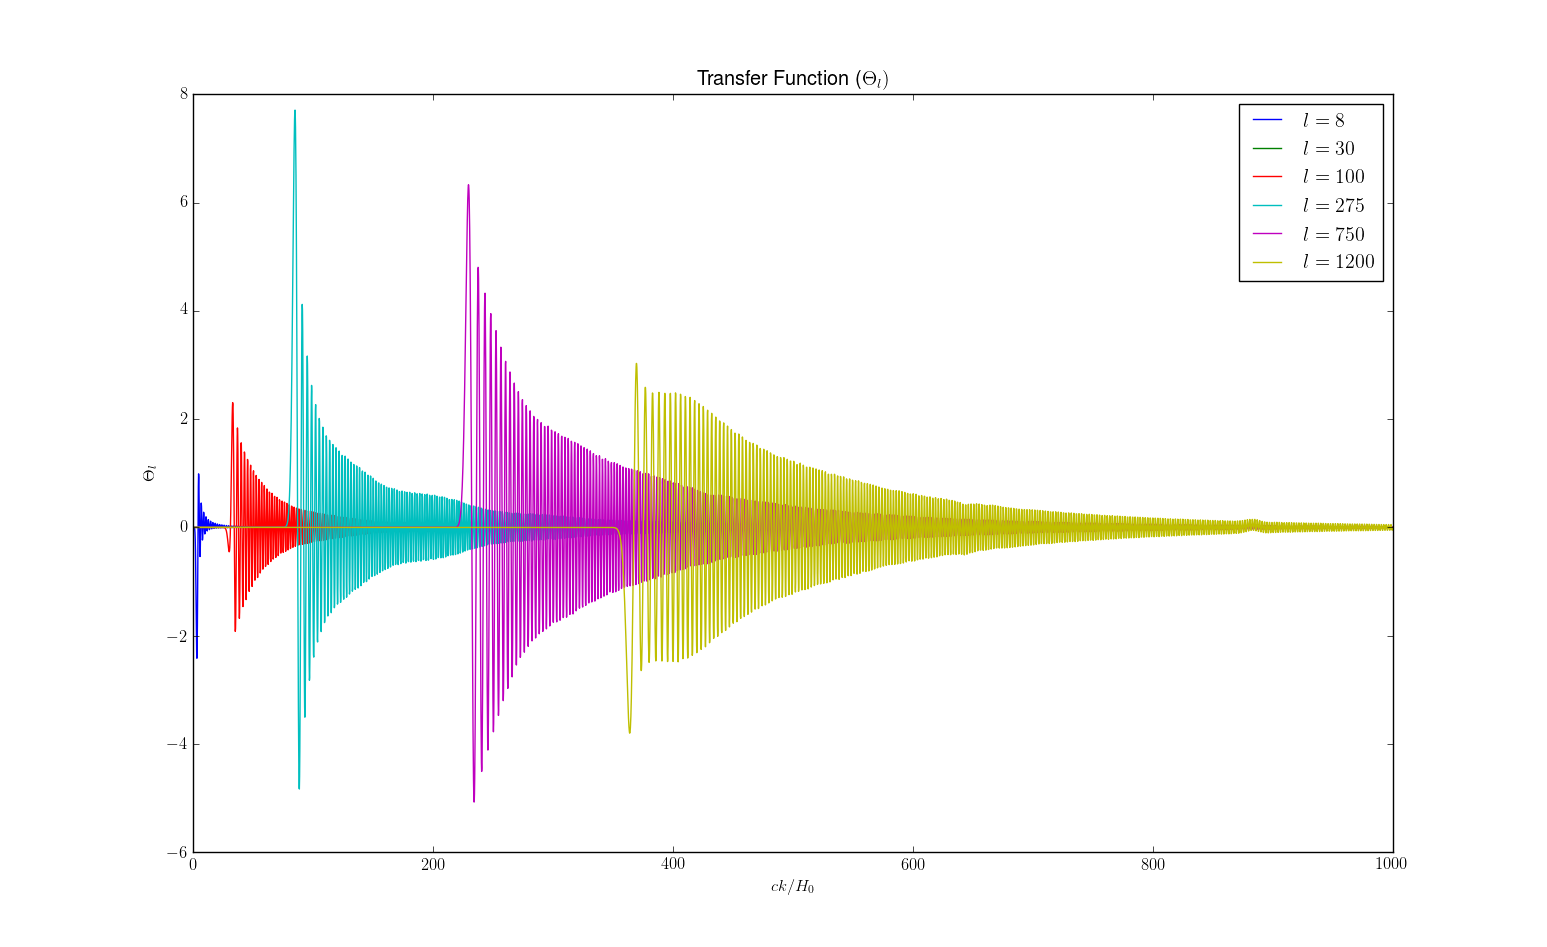
\includegraphics[width=\linewidth]{transfer_function_simulated}
\caption{The bevahior of the transfer function $\Theta_l$ for six different values of $l$ as a function of $k$. We see that for low $l$ values, the transfer function has a stronger contribution for lower $k$. As $l$ increases, so does the spread of the transfer function in $k$-space.}
\end{figure}

We see here that, as expected, different $l$ values for the transfer function $\Theta_l$ correspond to different Fourier scales. For larger $l$ values, the larger $k$ values contribute more. To inspect how the transfer function actually contributes to the values for $C_l$, we look at the integrand of equation \ref{eq:power}, namely the $ \dfrac{\Theta_l^2(k)}{k}$ portion which is shown below in figure \ref{fig:theta2}.\\

\subsection{$\Theta_l^2$}
In my simulations, I have run into the issue that for very low values of $l$, the magnitude of $C_l$ is very large with respect to other $C_l$s and is much larger than expected! We can see the results of this in the figure \ref{fig:theta2}. This has been a bit of a mystery for a few weeks and I am not sure at what point in our simple integration things break down. 

\begin{figure}[ht]\label{fig:theta2}
\centering
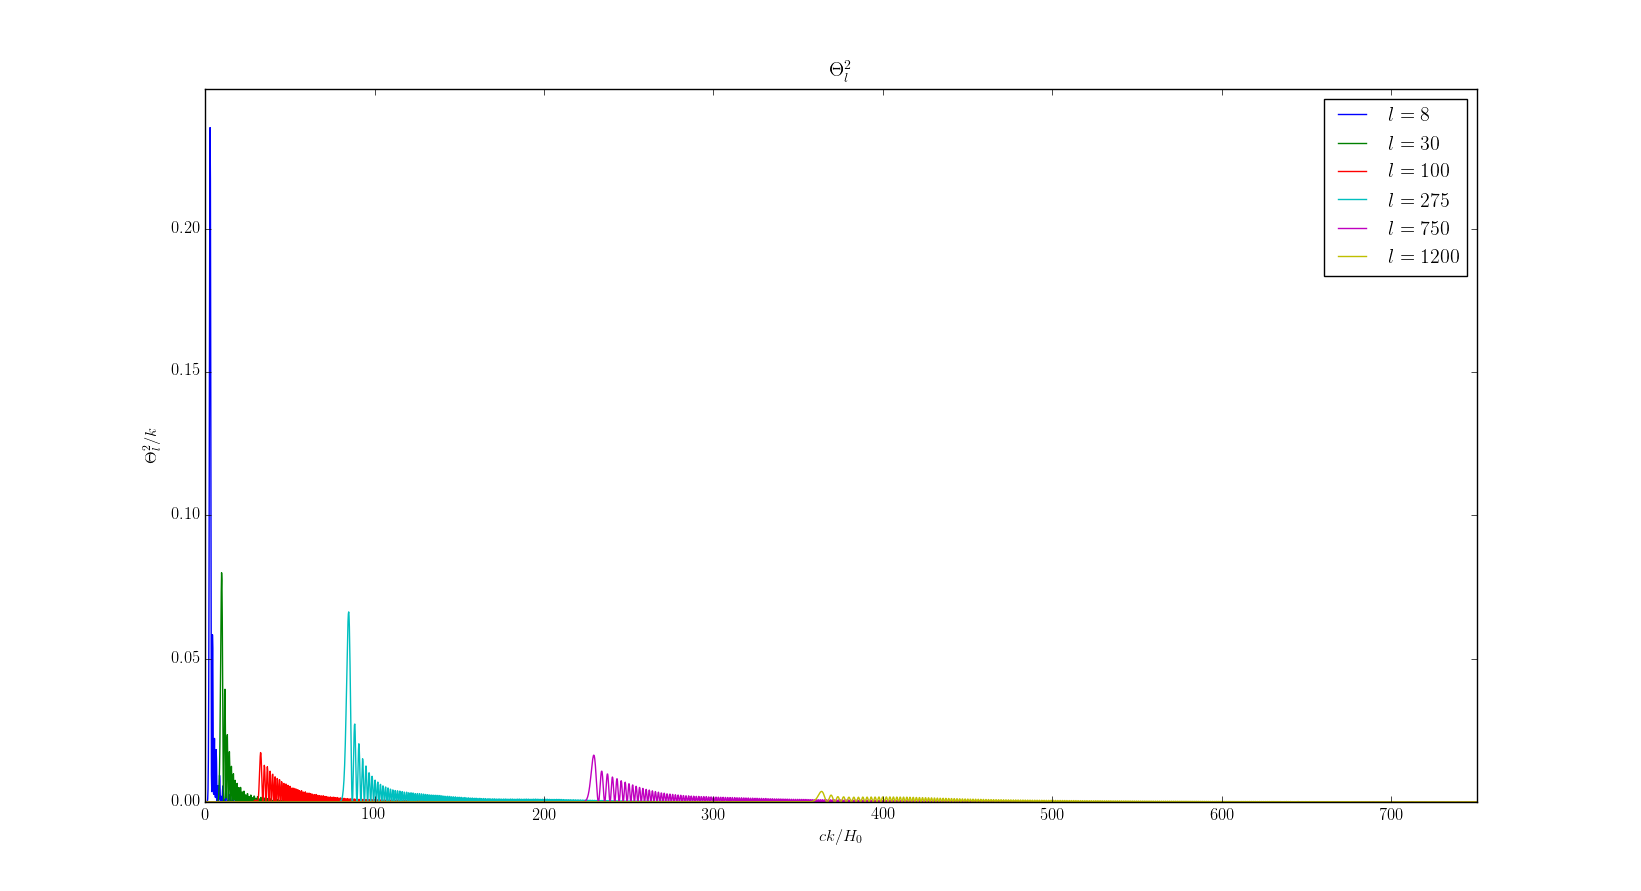
\includegraphics[width=\linewidth]{theta_squared}
\caption{The plot of $\Theta_l^2/k$ for the same six values of $l$, again plotted as a function of $k$. Similar behavior is shown here as in the above figure, however the see that for low $l$ we see a very strong contribution which is not what we would expect. It appears that there is an issue with this integrand.}
\end{figure}

We see that in the above plot, $\Theta_l^2$ for low $l$ values is far greater than when $l$ is at larger values with stronger contributions to the angular power spectrum like $l \simeq 200$. I believe that whatever causes this issue in $\Theta_l^2$ leads to the large low $l$, $C_l$ values that we are seen in the final results of our simulation.

\subsection{The Angular Power Spectrum $C_l$}

In this section the simulated angular power spectrum results are shown. The first plot shows the full simulation with the provided parameters, and the following plots show the simulation with different variations of some cosmological parameters. We have to keep in mind for these fits that we have neglected helium, neutrinos and polarization in our simulation, and we would not expect to have a perfect fit.\\

Below we see the results of changing the values for the relative radiation, dark matter and baryon densities, as well as the Hubble parameter $h$ in our simulation.\\

When changing the value of $\Omega_m$ we notice that for larger values the value of $C_l$ after the first peak generally increases (and decreases for lower $\Omega_m$. As well, it is seen in figure \ref{fig:omegm} that the following peaks in for the angular power spectrum move to lower $l$ values with a larger $\Omega_m$. The movement to lower $l$ is intuitive in the sense that for larger scales we would expect to see larger perturbations if there is more dark matter relative to the other cosmological parameters. Also, the changing value of $\Omega_m$ affects baryon loading; if there is more dark matter relative to baryons, the baryons "pull" the scaled oscillations of perturbation sizes less and the peaks increase. The inverse behavior is also seen in both of these cases.\\

In the case of changing the baryon densities, $\Omega_b$, we see the same baryon loading effect discussed in the previous paragraph. Namely, for lower densities of baryons relative to the dark matter density we notice a decrease in the effect of baryon loading. When $\Omega_b$ is increased, we see that the values of the peaks decrease.\\

We run into some of the drawbacks of our simulation when we alter the value of $\Omega_r$. In reality, if we change the radiation density (or the matter densities), the time at which recombination happens changes. In our model, however, we set the recombination period at fixed points in time. However, we still see the results of some of these affects as the value of $\Omega_r$ affects the duration of tight coupling and therefore at which time perturbations of larger size can continue to grow. As seen in figure \ref{fig:omegr}, the peaks of $C_l$ move to larger $l$ values with larger radiation densities. We also observe a rebound in the $C_l$ values following the first peak that leads to a larger second peak for larger radiation densities.\\

The final parameter adjustment that was investigated was the Hubble parameter $h$. The value was changed less than $10\%$ here, and we see that the effects of these small changes were minor. We notice though, that the height of the following peaks increase for larger $h$ and decrease for smaller $h$.

\begin{figure}[ht]\label{fig:sim}
\centering
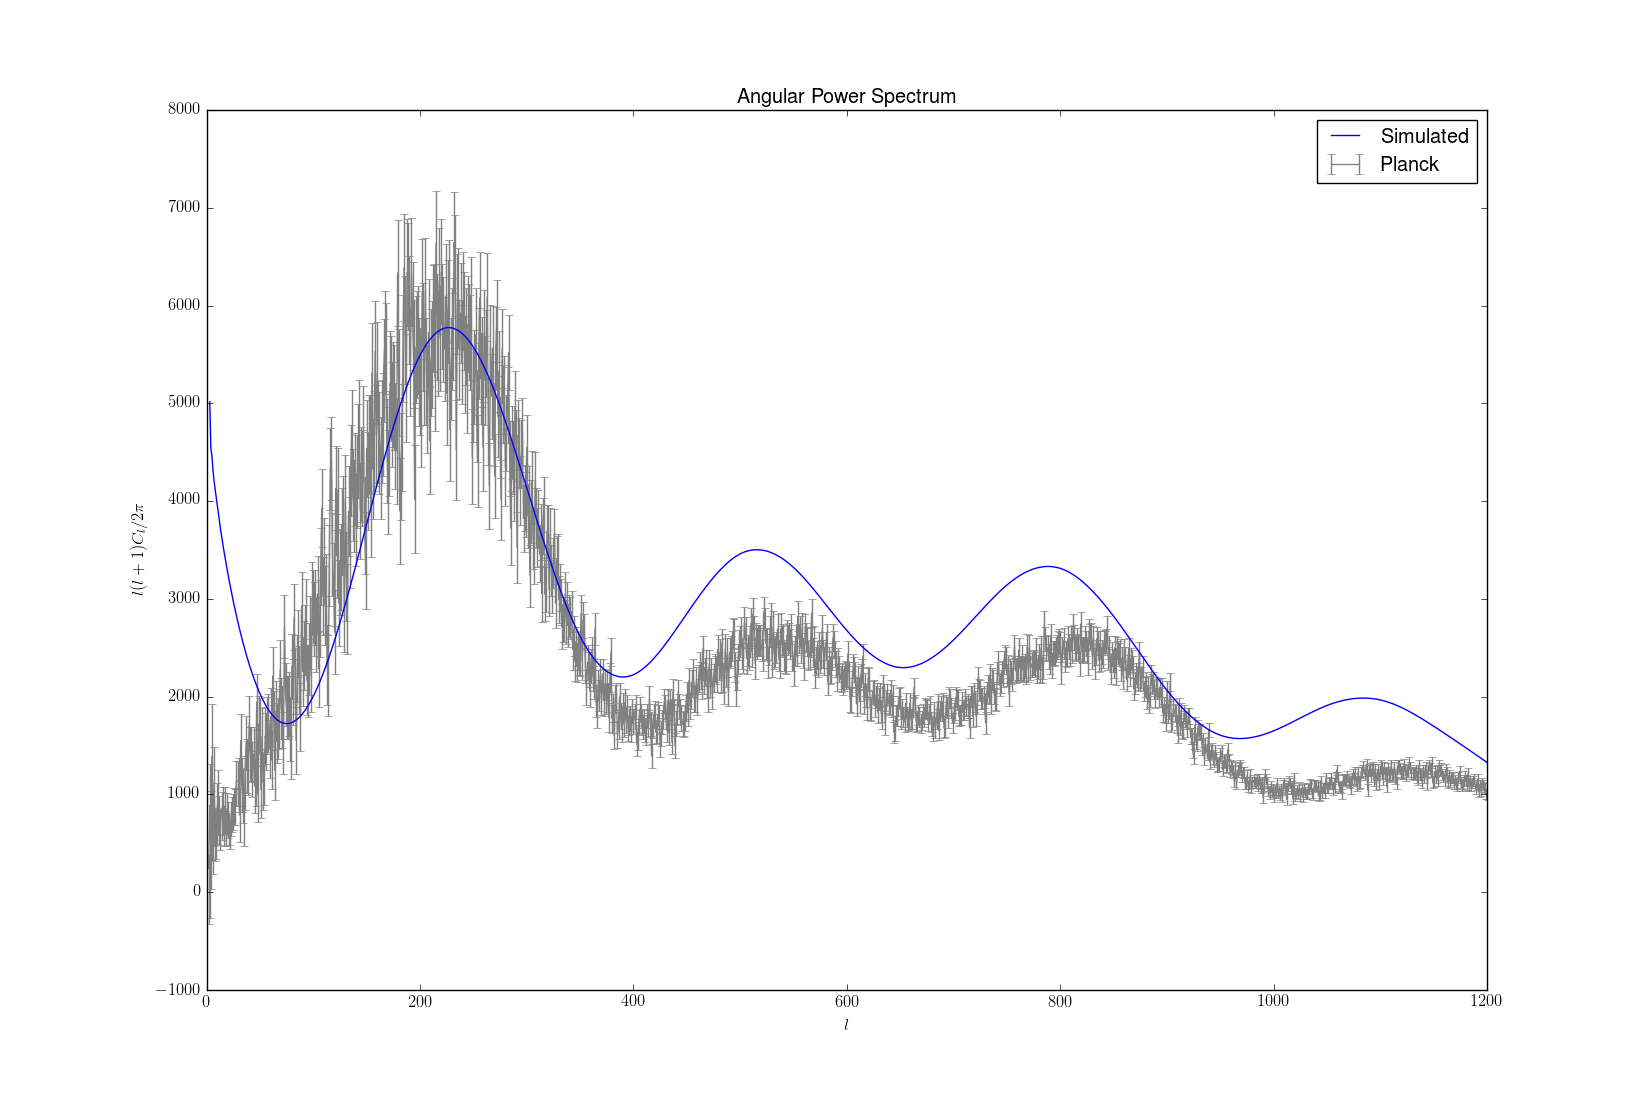
\includegraphics[width=\linewidth]{C_l_simulated}
\caption{Here is the full CMB angular power spectrum results plotted against the most recent Planck collaboration angular power spectrum estimates with error bars included.}
\end{figure}

\begin{figure}[ht]\label{fig:omegm}
\centering
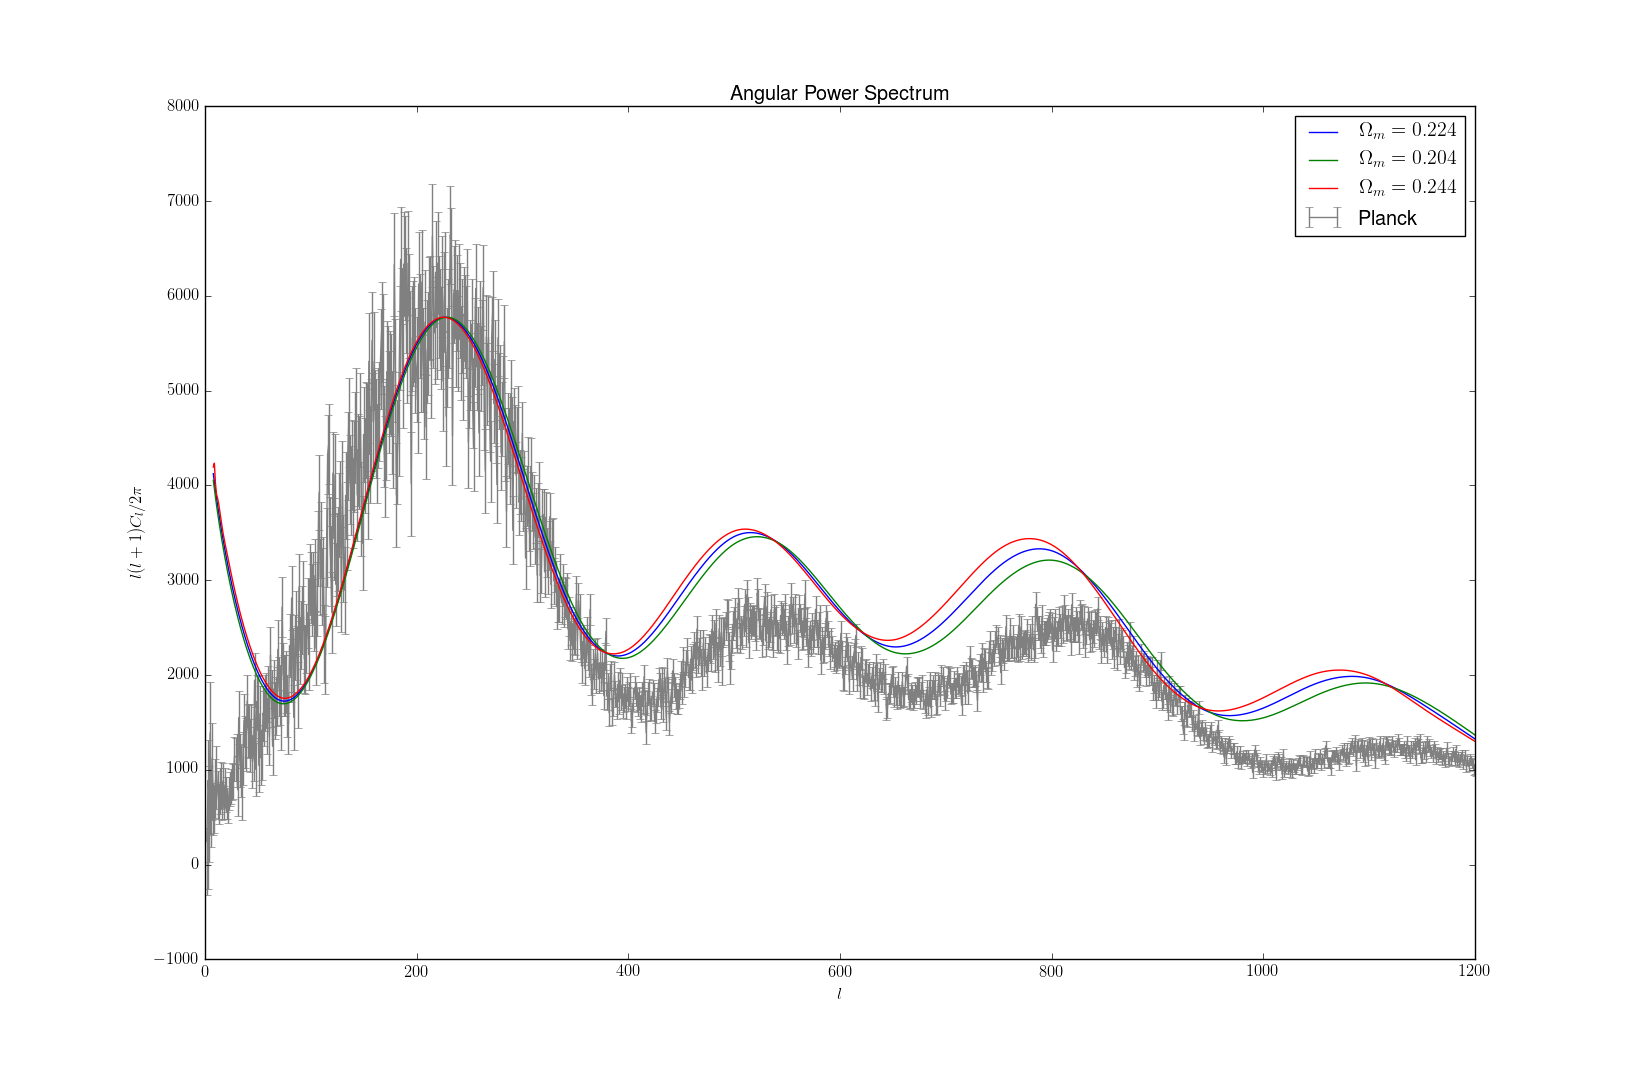
\includegraphics[width=\linewidth]{C_l_omega_m}
\caption{Adjustments of the value of $\Omega_m$ in the Angular Power Spectrum simulation.}
\end{figure}

\begin{figure}[ht]\label{fig:omegb}
\centering
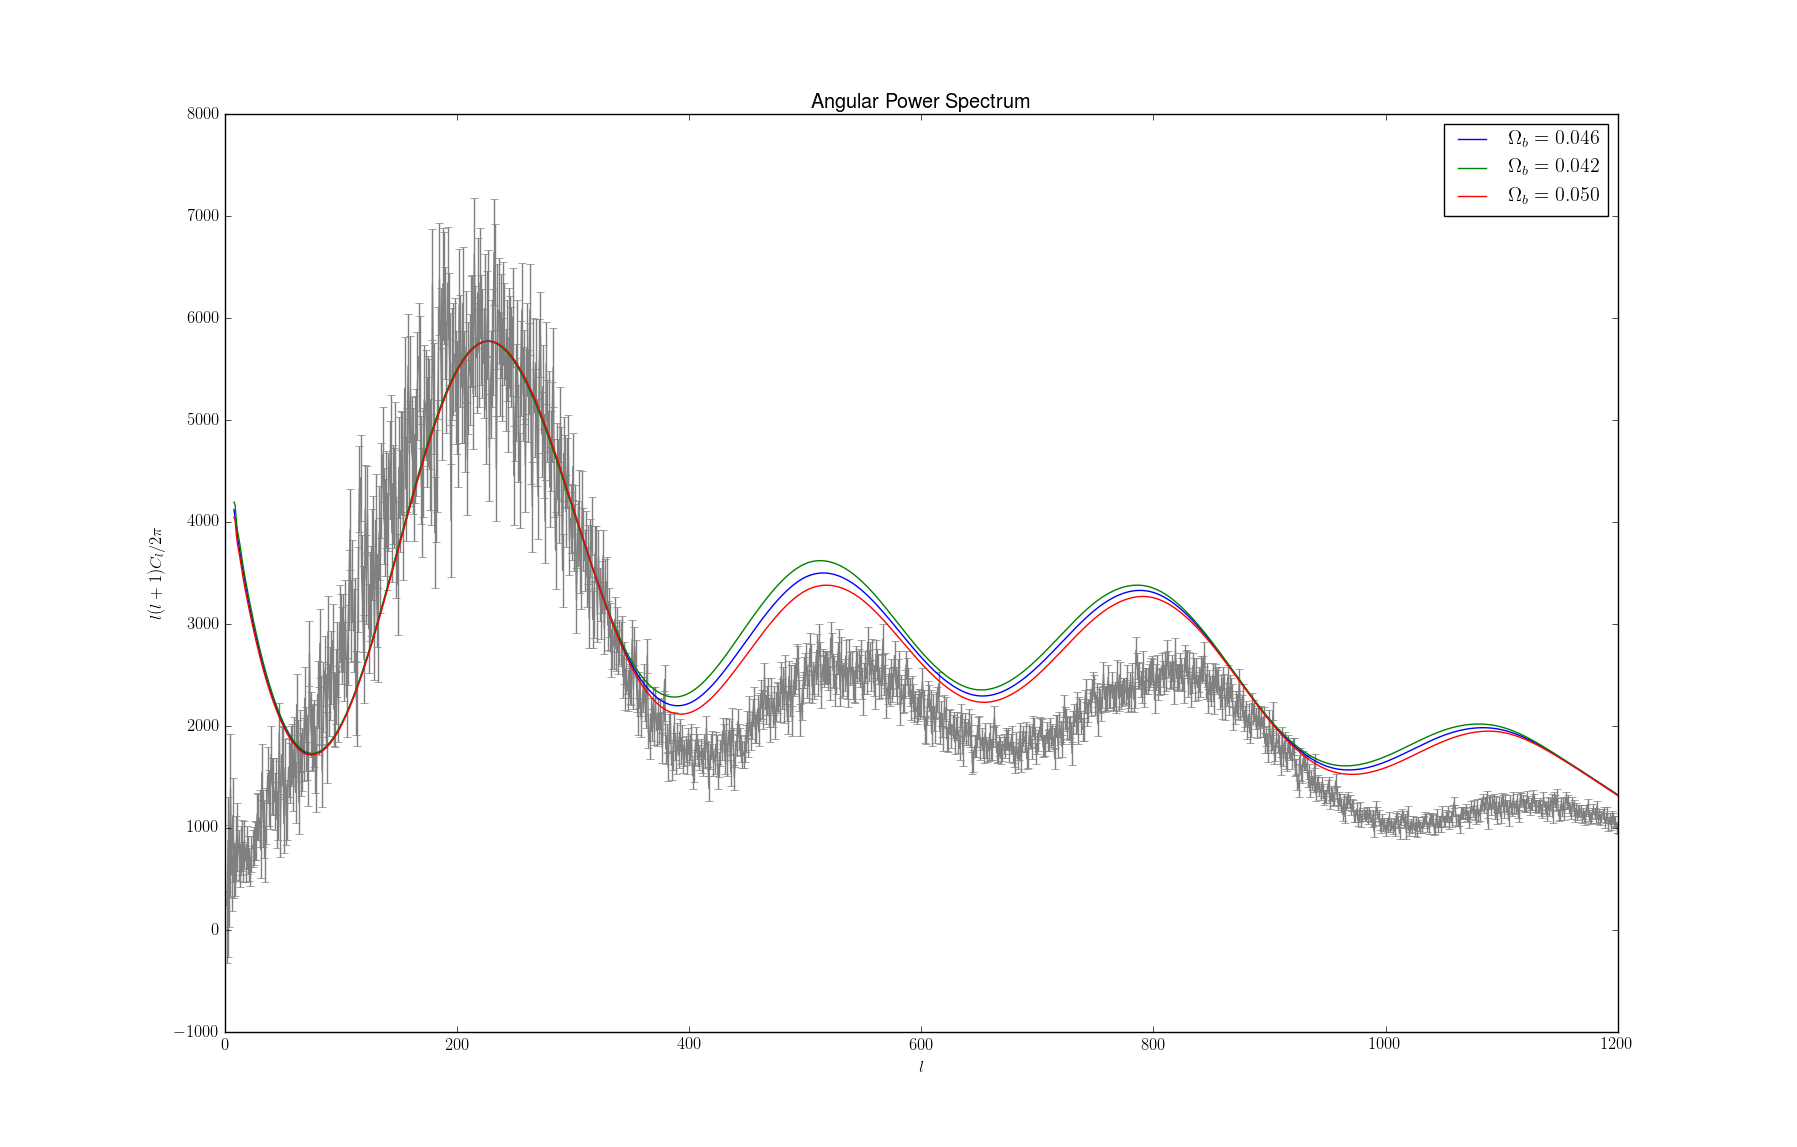
\includegraphics[width=\linewidth]{C_l_omega_b}
\caption{Adjustments of the value of $\Omega_b$ in the Angular Power Spectrum simulation.}
\end{figure}

\begin{figure}[ht]\label{fig:omegr}
\centering
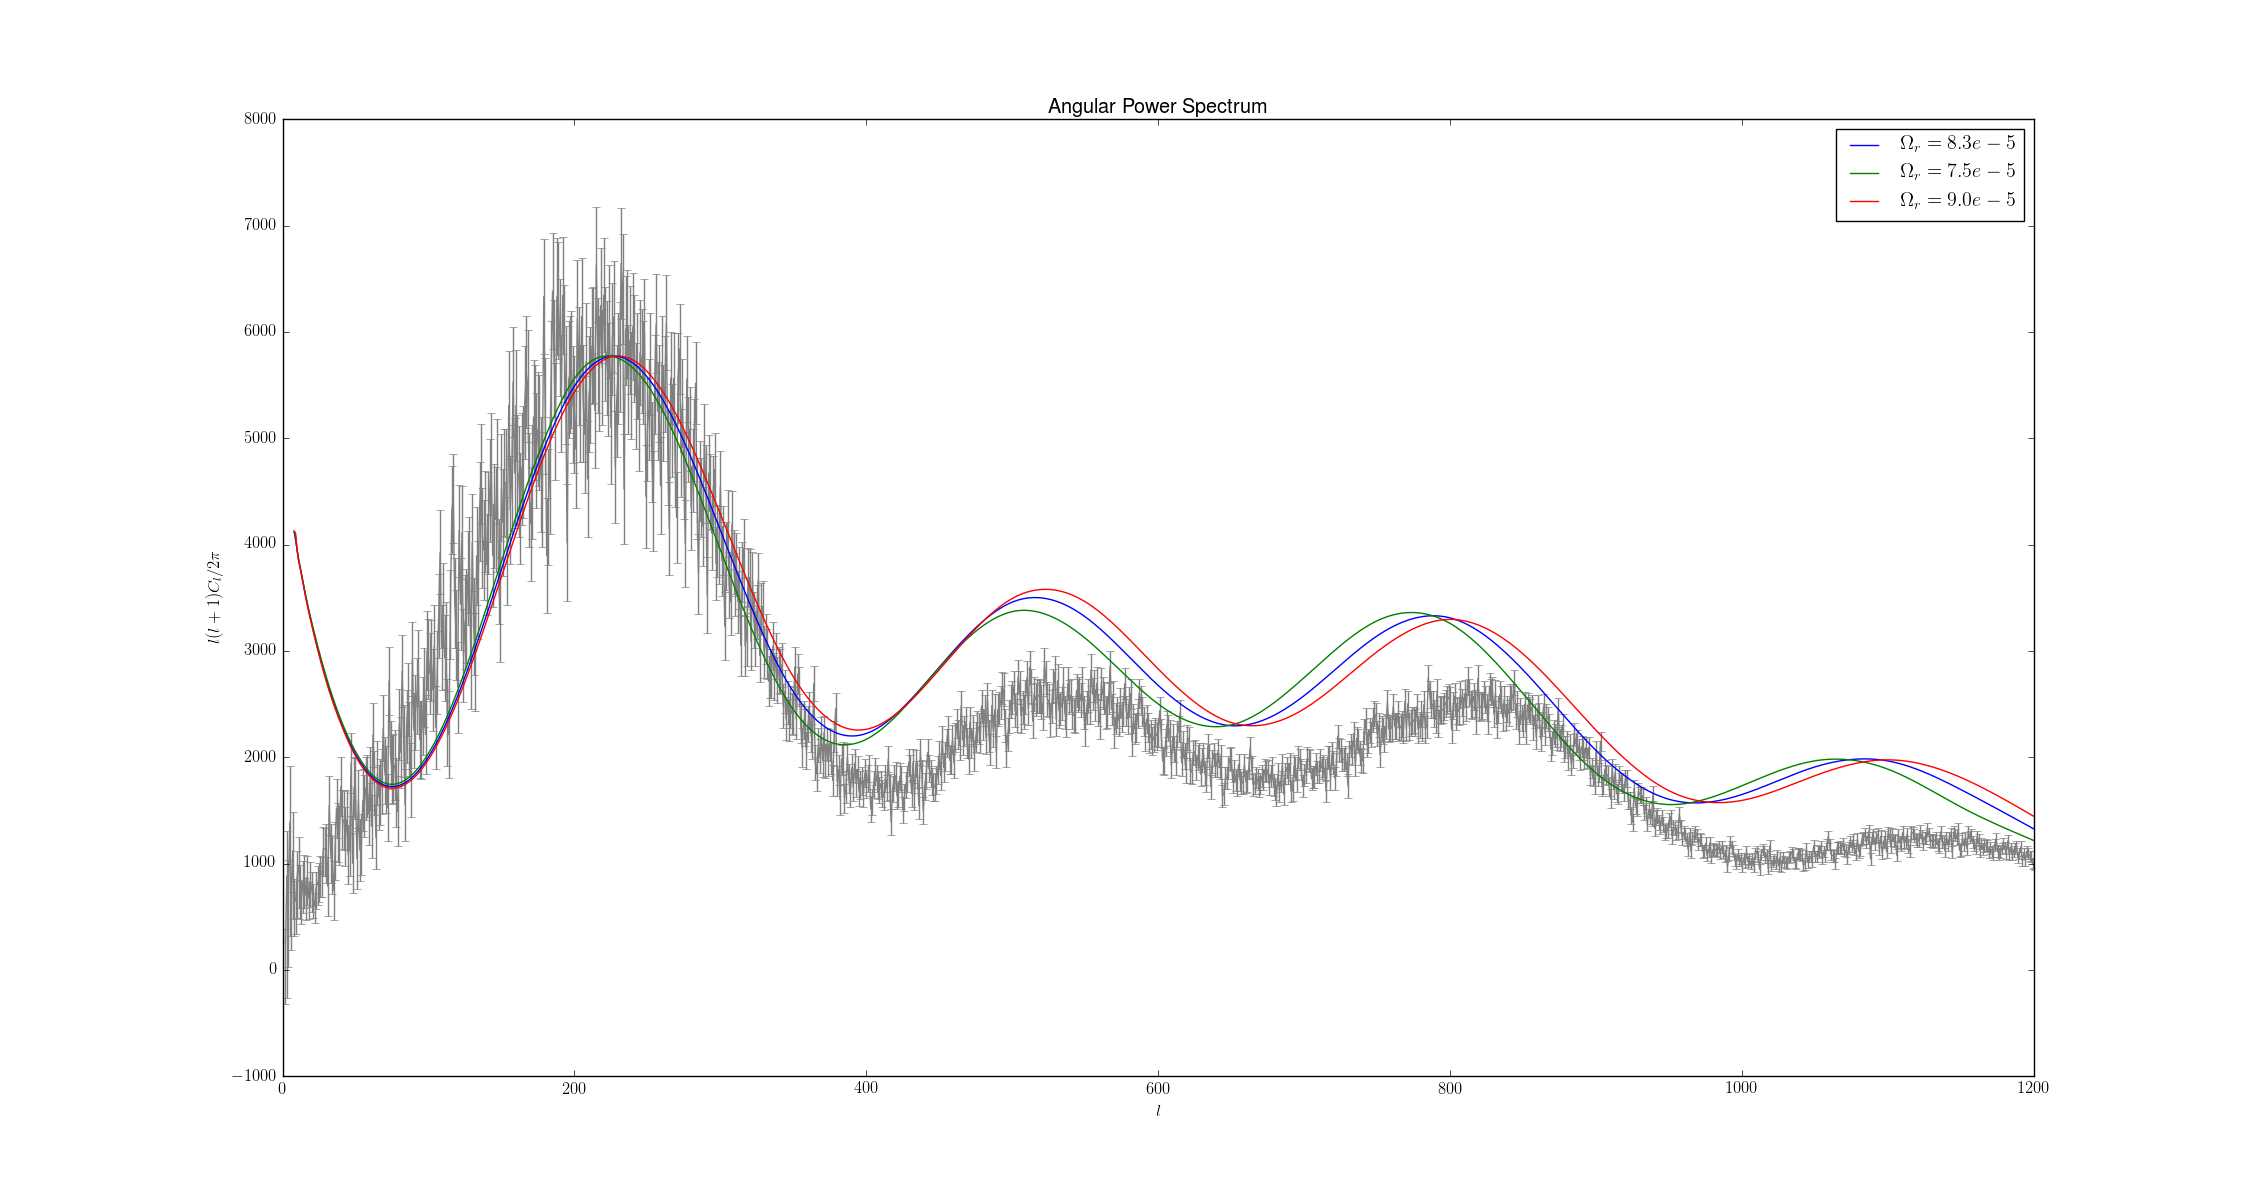
\includegraphics[width=\linewidth]{C_l_omega_r}
\caption{Adjustments of the value of $\Omega_r$ in the Angular Power Spectrum simulation.}
\end{figure}

\begin{figure}[ht]\label{fig:h}
\centering
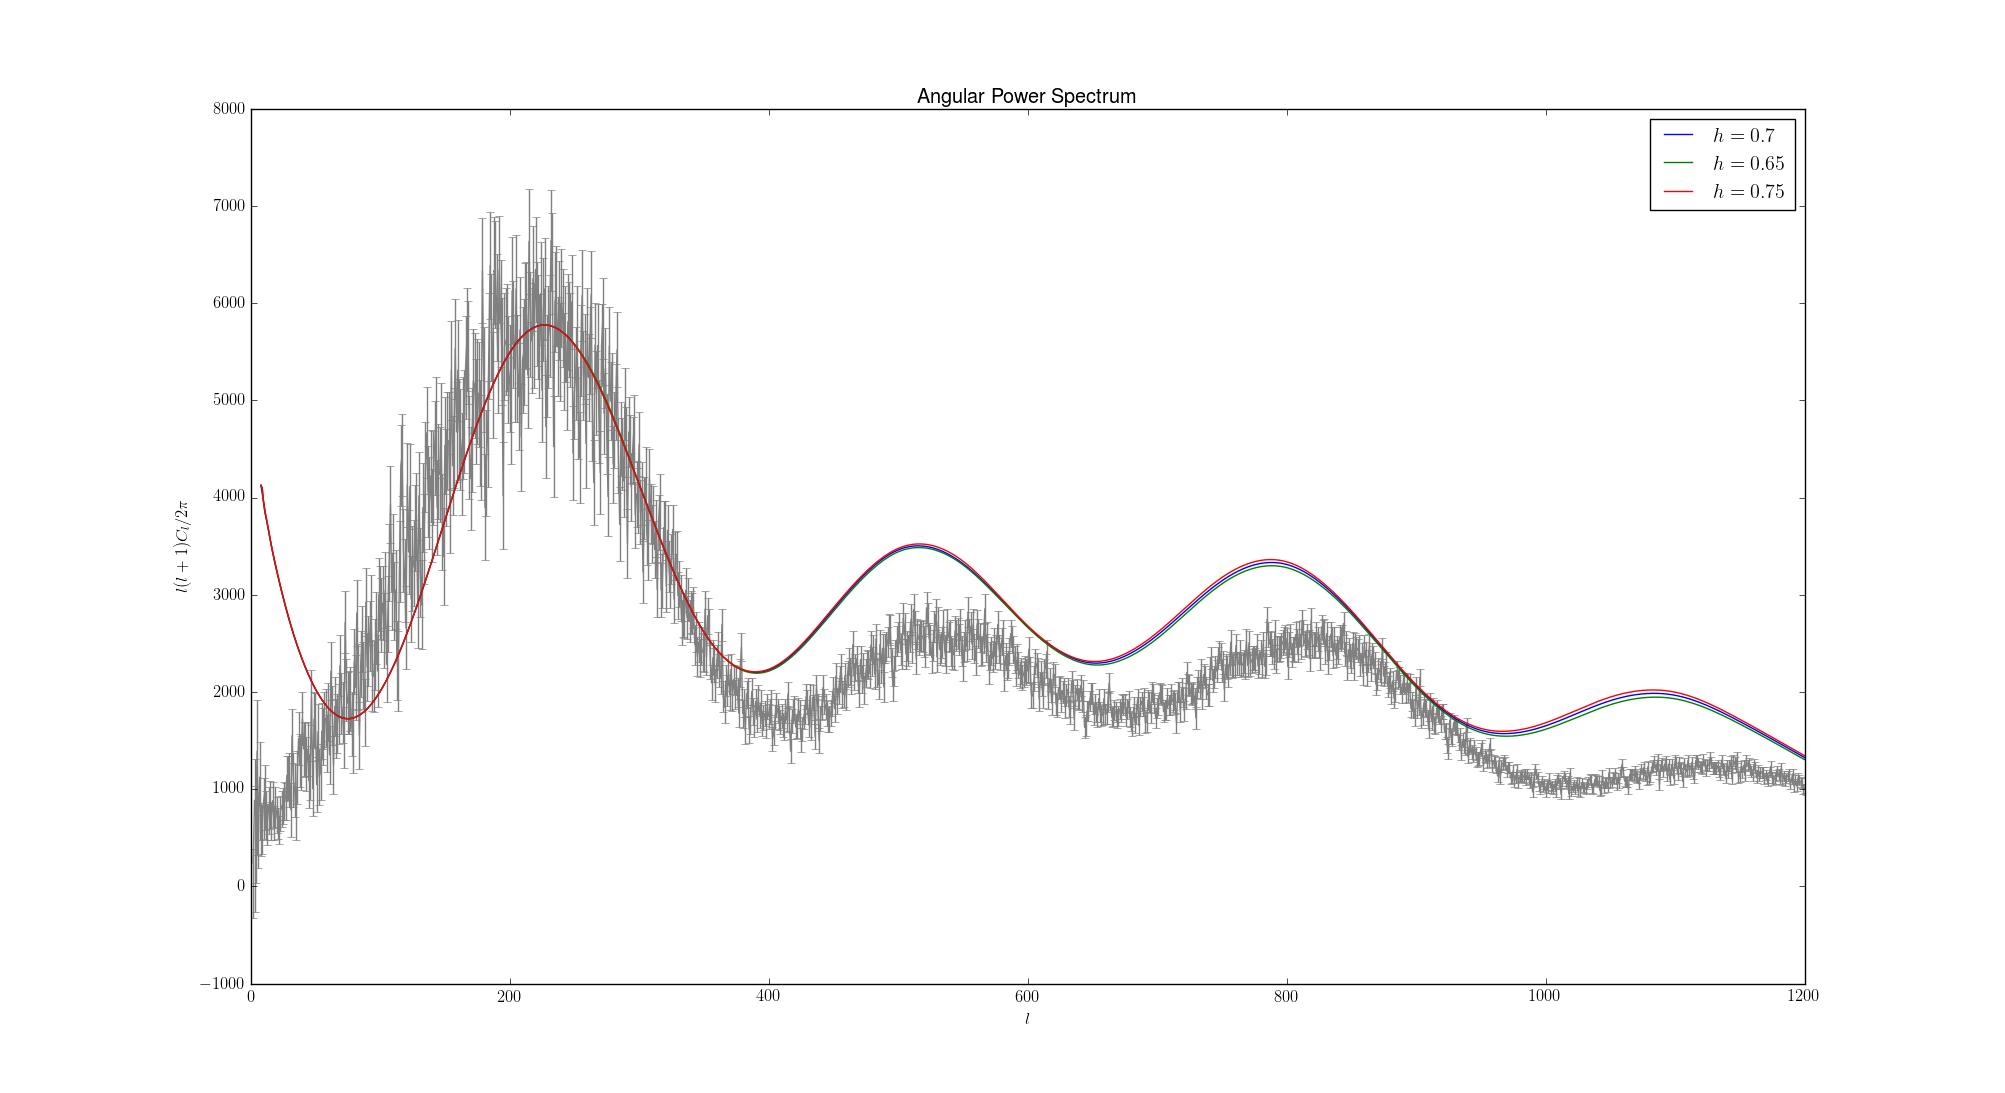
\includegraphics[width=\linewidth]{C_l_h}
\caption{Adjustments of the value of $h$ in the Angular Power Spectrum simulation.}
\end{figure}

\end{document}